\documentclass[12pt, a4paper]{article}

\usepackage[margin=2.5cm]{geometry}
\usepackage{graphicx}
\usepackage{hyperref}
\usepackage{booktabs}
\usepackage{array}
\usepackage{parskip}
\usepackage{titlesec}
\usepackage{xcolor}
\usepackage{fontenc}
\usepackage{inputenc}
\usepackage{tikz}
\usepackage{float}
\usepackage{enumitem}
\usetikzlibrary{shapes.geometric, arrows.meta, positioning, fit, backgrounds, calc, decorations.pathreplacing}

% Tighter list spacing
\setlist[itemize]{noitemsep, topsep=3pt}
\setlist[enumerate]{noitemsep, topsep=3pt}

% Reduce space before/after figures
\setlength{\floatsep}{6pt}
\setlength{\textfloatsep}{8pt}
\setlength{\intextsep}{6pt}

% Reduce section spacing
\titlespacing*{\section}{0pt}{10pt}{4pt}
\titlespacing*{\subsection}{0pt}{6pt}{3pt}

\hypersetup{
    colorlinks=true,
    linkcolor=blue,
    urlcolor=blue,
    citecolor=blue
}

\titleformat{\section}{\large\bfseries}{}{0em}{}[\titlerule]
\titleformat{\subsection}{\normalsize\bfseries}{}{0em}{}

\definecolor{xenpurple}{RGB}{88, 44, 131}
\definecolor{qubesblue}{RGB}{41, 128, 185}
\definecolor{securegreen}{RGB}{39, 174, 96}
\definecolor{warnorange}{RGB}{230, 126, 34}
\definecolor{lightgray}{RGB}{245, 245, 245}

\begin{document}

%---------------------------------------------------------------
% COVER PAGE
%---------------------------------------------------------------
\begin{titlepage}
    \centering
    \vspace*{0.5cm}
    \includegraphics[width=0.25\textwidth]{gsoc_logo.png}\\[0.3cm]
    {\large\textbf{Google Summer of Code 2026}}\\[0.2cm]
    {\large @}\\[0.5cm]
    \includegraphics[width=0.35\textwidth]{images.png}\\[0.2cm]
    {\large\textbf{QUBES OS}}\\
    {\small\textit{A Reasonably Secure Operating System}}\\[1cm]
    {\LARGE\textbf{Proposal}}\\[0.3cm]
    {\LARGE\textbf{Secure Boot Support for Qubes OS}}\\[1.5cm]
    {\large\textbf{Harshit Bhalani}}\\[0.2cm]
    {\normalsize March 29, 2026}
    \vfill
\end{titlepage}

%---------------------------------------------------------------
% TABLE OF CONTENTS
%---------------------------------------------------------------
\tableofcontents
\newpage

%---------------------------------------------------------------
% APPLICANT TABLE
%---------------------------------------------------------------
\begin{table}[h]
\centering
\begin{tabular}{>{\bfseries}p{4cm} p{9cm}}
\toprule
Applicant    & Harshit Bhalani \\
Email        & \href{mailto:harshitbhalani6@gmail.com}{harshitbhalani6@gmail.com} \\
GitHub       & \href{https://github.com/Harshit6-b}{github.com/Harshit6-b} \\
Mentor       & Marek Marczykowski-G\'{o}recki \\
Organization & Invisible Things Lab / Qubes OS \\
Size         & 175 hours \\
Time Zone    & UTC+05:30 (IST) \\
\bottomrule
\end{tabular}
\end{table}

%---------------------------------------------------------------
% 1. INTRODUCTION
%---------------------------------------------------------------
\section{Introduction}

Qubes OS builds its entire security model on hardware-enforced isolation. Yet this isolation only begins \textit{after} the bootloader runs; the boot chain itself is unsigned and unverified. An attacker with physical access, a compromised firmware update, or a supply-chain compromise can silently replace Xen, the Dom0 kernel, or boot parameters before Qubes initialises. UEFI Secure Boot is precisely the mechanism designed to close this gap.

\begin{figure}[H]
\centering
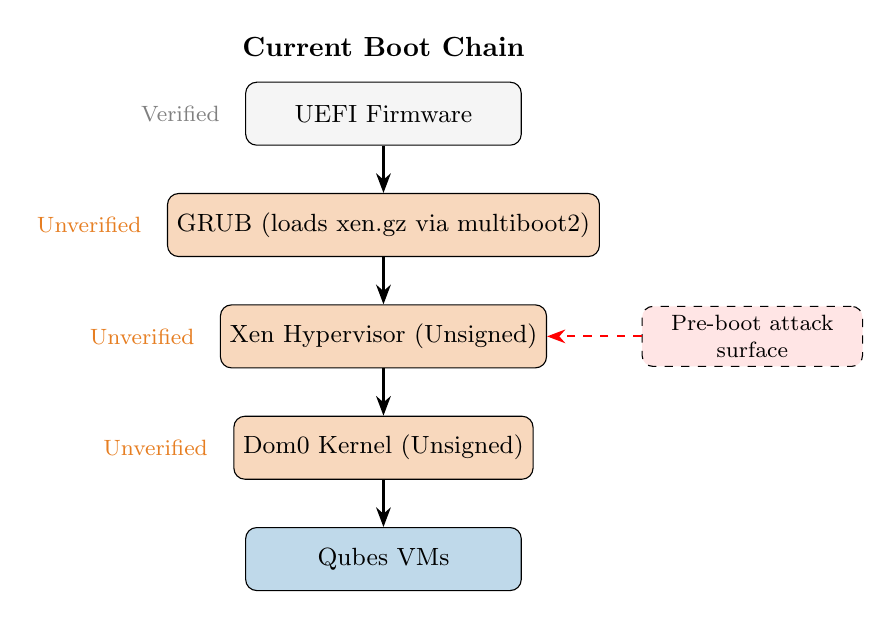
\begin{tikzpicture}[
    node distance=0.6cm,
    every node/.style={font=\small},
    block/.style={rectangle, draw, rounded corners, minimum width=3.5cm, minimum height=0.8cm, align=center},
    attack/.style={rectangle, draw, dashed, fill=red!10, rounded corners, minimum width=2.8cm, minimum height=0.6cm, align=center, font=\footnotesize},
    arrow/.style={-{Stealth[length=2.5mm]}, thick}
]
\node[block, fill=lightgray] (uefi) {UEFI Firmware};
\node[block, fill=warnorange!30, below=of uefi] (grub) {GRUB (loads xen.gz via multiboot2)};
\node[block, fill=warnorange!30, below=of grub] (xen) {Xen Hypervisor (Unsigned)};
\node[block, fill=warnorange!30, below=of xen] (dom0) {Dom0 Kernel (Unsigned)};
\node[block, fill=qubesblue!30, below=of dom0] (qubes) {Qubes VMs};
\node[attack, right=1.2cm of xen] (atk) {Pre-boot attack\\surface};
\draw[arrow] (uefi) -- (grub);
\draw[arrow] (grub) -- (xen);
\draw[arrow] (xen) -- (dom0);
\draw[arrow] (dom0) -- (qubes);
\draw[-{Stealth}, dashed, red, thick] (atk) -- (xen);
\node[left=0.2cm of uefi, font=\footnotesize, text=gray] {Verified};
\node[left=0.2cm of grub, font=\footnotesize, text=warnorange] {Unverified};
\node[left=0.2cm of xen, font=\footnotesize, text=warnorange] {Unverified};
\node[left=0.2cm of dom0, font=\footnotesize, text=warnorange] {Unverified};
\node[above=0.2cm of uefi, font=\bfseries] {Current Boot Chain};
\end{tikzpicture}
\caption{Current Qubes boot chain. GRUB loads Xen via multiboot2; none of these components are cryptographically verified.}
\label{fig:current-boot}
\end{figure}

Since recent releases, Xen supports a ``unified EFI boot'' model in which Xen, the Dom0 kernel, initramfs, and boot parameters are bundled into a single PE/COFF binary (UKI) that can be signed as one unit and verified by UEFI firmware. Qubes R4.3 will ship pre-built unified \texttt{xen.efi} binaries via \href{https://github.com/QubesOS/qubes-vmm-xen-unified}{\texttt{qubes-vmm-xen-unified}}, but the user-facing tooling to sign these binaries, generate keys, handle updates, and provide fallback recovery does not yet exist.

A Qubes user who wants Secure Boot today faces a fully manual process: no signing tooling, no key generation guidance, no update integration, and no fallback path. This project builds that end-to-end, extending \texttt{qubes-vmm-xen-unified} with signing, key management, and update hooks. See \href{https://github.com/QubesOS/qubes-issues/issues/4371}{issue \#4371} and \href{https://github.com/QubesOS/qubes-issues/issues/8206}{issue \#8206}.

%---------------------------------------------------------------
% 2. PROJECT GOALS
%---------------------------------------------------------------
\section{Project Goals}

\subsection*{Committed Deliverables}
\begin{enumerate}
    \item \textbf{UKI Signing Tool (\texttt{qubes-uki-sign}):} Signs the pre-built unified \texttt{xen.efi} from \texttt{qubes-vmm-xen-unified} with user-generated keys, configurable via \texttt{/etc/qubes/secureboot.conf}
    \item \textbf{Key Management (\texttt{qubes-sb-keygen}):} Generates a PK/KEK/db key hierarchy with configurable parameters, produces \texttt{.auth} files, and provides step-by-step enrollment instructions
    \item \textbf{Update Integration:} A post-transaction RPM hook that automatically re-signs the UKI whenever \texttt{qubes-vmm-xen-unified} or \texttt{kernel-qubes-dom0} packages are updated, with \texttt{qubes-pecheck} verification before installation
    \item \textbf{Fallback Recovery (\texttt{qubes-uki-promote-fallback}):} A fallback UKI (\texttt{qubes-fallback.efi}) built from a last-known-good snapshot, registered as a lower-priority UEFI boot entry
    \item \textbf{Documentation:} Key generation, signing workflow, enrollment, update integration, and recovery procedures
\end{enumerate}

\textbf{Starter Task (Pre-GSoC):} Fix two \texttt{qubes-pecheck} false positives identified during analysis of real-world EFI binaries. Patches submitted during community bonding.

\subsection*{Explicitly Out of Scope}
\begin{itemize}
    \item Microsoft CA signing path (blocked by Xen's missing SBAT support and NX\_COMPAT issues)
    \item TPM-based remote attestation or PCR-based sealing
    \item Multi-kernel support beyond the active Dom0 kernel
\end{itemize}

%---------------------------------------------------------------
% 3. IMPLEMENTATION
%---------------------------------------------------------------
\section{Implementation Details}

\subsection{Secure Boot Architecture Overview}

\begin{figure}[H]
\centering
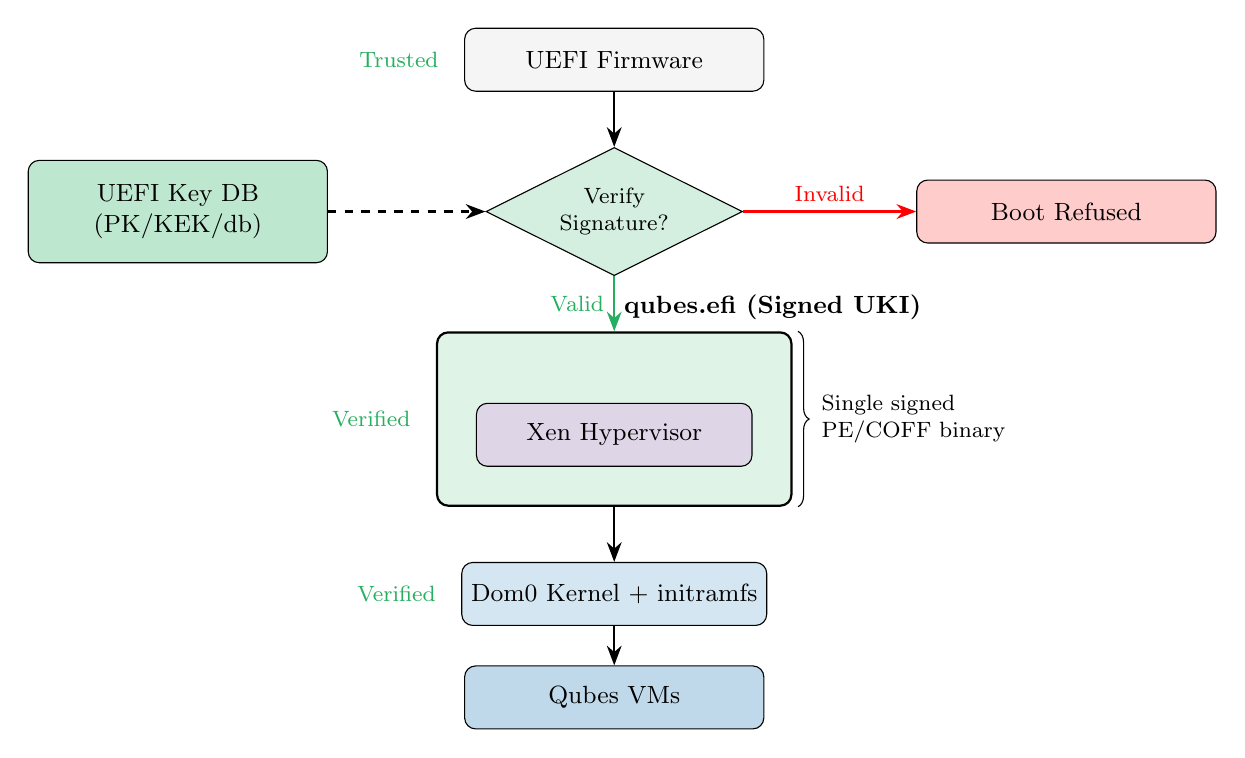
\begin{tikzpicture}[
    node distance=0.55cm and 1.5cm,
    every node/.style={font=\small},
    block/.style={rectangle, draw, rounded corners, minimum width=3.8cm, minimum height=0.8cm, align=center},
    verify/.style={diamond, draw, aspect=2, fill=securegreen!20, minimum width=2cm, align=center, font=\footnotesize},
    arrow/.style={-{Stealth[length=2.5mm]}, thick},
    signed/.style={rectangle, draw, thick, fill=securegreen!15, rounded corners}
]
\node[block, fill=lightgray] (uefi) {UEFI Firmware};
\node[verify, below=0.7cm of uefi] (check) {Verify\\Signature?};
\node[signed, below=0.7cm of check, minimum width=4.5cm, minimum height=2.2cm] (uki) {};
\node[above=0.3cm,right] at (uki.north) {\textbf{qubes.efi (Signed UKI)}};
\node[block, fill=xenpurple!20, minimum width=3.5cm] at ([yshift=-0.2cm,]uki.center) (xen) {Xen Hypervisor};
\node[block, fill=qubesblue!20, below=0.7cm of uki] (dom0) {Dom0 Kernel + initramfs};
\node[block, fill=qubesblue!30, below=0.5cm of dom0] (qubes) {Qubes VMs};
\node[block, fill=red!20, right=2.2cm of check] (fail) {Boot Refused};
\node[block, fill=securegreen!30, left=2cm of check, minimum height=1.3cm] (keys) {UEFI Key DB\\(PK/KEK/db)};
\draw[arrow] (uefi) -- (check);
\draw[arrow, securegreen] (check) -- node[left, font=\footnotesize] {Valid} (uki);
\draw[arrow, red] (check) -- node[above, font=\footnotesize] {Invalid} (fail);
\draw[arrow] (uki) -- (dom0);
\draw[arrow] (dom0) -- (qubes);
\draw[arrow, dashed] (keys) -- (check);
\draw[decorate, decoration={brace, amplitude=4pt, raise=2pt}]
    (uki.north east) -- (uki.south east)
    node[midway, right=7pt, font=\footnotesize, align=left] {Single signed\\PE/COFF binary};
\node[left=0.2cm of uefi, font=\footnotesize, text=securegreen] {Trusted};
\node[left=0.2cm of uki, font=\footnotesize, text=securegreen] {Verified};
\node[left=0.2cm of dom0, font=\footnotesize, text=securegreen] {Verified};
\end{tikzpicture}
\caption{Secure Boot architecture. UEFI verifies the signed UKI against enrolled keys before executing any Qubes code.}
\label{fig:secure-boot}
\end{figure}

\subsection{UKI Structure and Assembly}

The \texttt{qubes-vmm-xen-unified} package produces a unified \texttt{xen.efi} by embedding Dom0 kernel, initramfs, and boot parameters into the existing Xen EFI binary using \texttt{objcopy --add-section} after Xen's \texttt{.pad} section:

\begin{table}[H]
\centering
\small
\begin{tabular}{>{\ttfamily}p{2.2cm} p{6.5cm} p{3.2cm}}
\toprule
\normalfont\textbf{Section} & \textbf{Contents} & \textbf{Source} \\
\midrule
(Xen native)  & Xen hypervisor code and data sections & xen.efi (base) \\
.pad         & Alignment padding (assembly point) & xen.efi (base) \\
.cmdline     & Xen and kernel command-line & Embedded \\
.initrd      & initramfs + microcode blobs & Embedded \\
.linux       & Dom0 kernel (vmlinuz) & Embedded \\
\bottomrule
\end{tabular}
\end{table}

\begin{figure}[H]
\centering
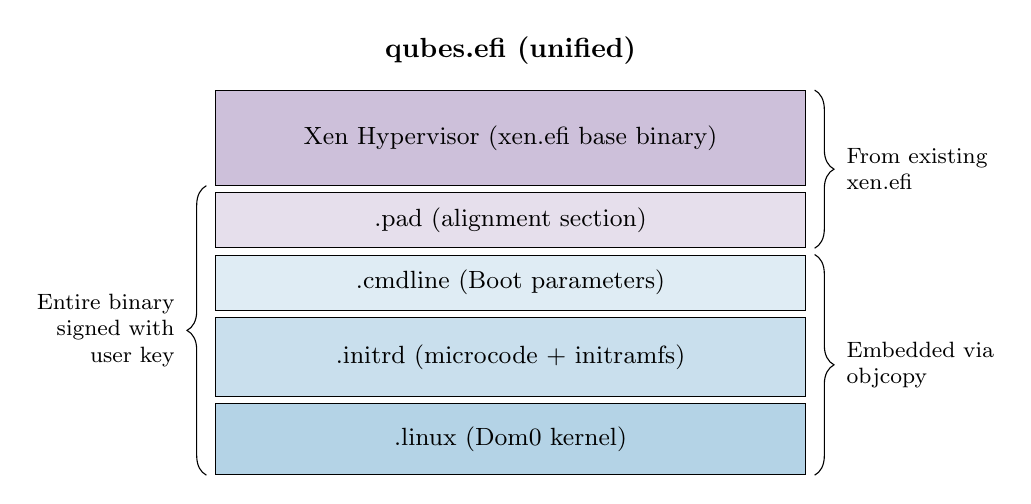
\begin{tikzpicture}[
    every node/.style={font=\small},
    section/.style={rectangle, draw, minimum width=7.5cm, minimum height=0.7cm, align=center}
]
\node[section, fill=xenpurple!30, minimum height=1.2cm] (xen) {Xen Hypervisor (xen.efi base binary)};
\node[section, fill=xenpurple!15, below=0.08cm of xen] (pad) {.pad (alignment section)};
\node[section, fill=qubesblue!15, below=0.08cm of pad] (cmdline) {.cmdline (Boot parameters)};
\node[section, fill=qubesblue!25, below=0.08cm of cmdline, minimum height=1.0cm] (initrd) {.initrd (microcode + initramfs)};
\node[section, fill=qubesblue!35, below=0.08cm of initrd, minimum height=0.9cm] (linux) {.linux (Dom0 kernel)};
\draw[decorate, decoration={brace, amplitude=7pt, raise=3pt}]
    (xen.north east) -- (pad.south east)
    node[midway, right=11pt, font=\footnotesize, align=left] {From existing\\xen.efi};
\draw[decorate, decoration={brace, amplitude=7pt, raise=3pt}]
    (cmdline.north east) -- (linux.south east)
    node[midway, right=11pt, font=\footnotesize, align=left] {Embedded via\\objcopy};
\draw[decorate, decoration={brace, amplitude=7pt, mirror, raise=3pt}]
    (xen.south west) -- (linux.south west)
    node[midway, left=11pt, font=\footnotesize, align=right] {Entire binary\\signed with\\user key};
\node[above=0.2cm of xen, font=\bfseries] {qubes.efi (unified)};
\end{tikzpicture}
\caption{UKI structure. Sections are embedded into the existing Xen EFI binary, then the whole binary is signed.}
\label{fig:uki-structure}
\end{figure}

This project does \textbf{not} re-implement UKI assembly; \texttt{qubes-vmm-xen-unified} already handles that. The \texttt{qubes-uki-sign} tool takes the pre-built unified binary and signs it with the user's db key using \texttt{sbsign}.

\subsection{Key Hierarchy and Management}

\begin{figure}[H]
\centering
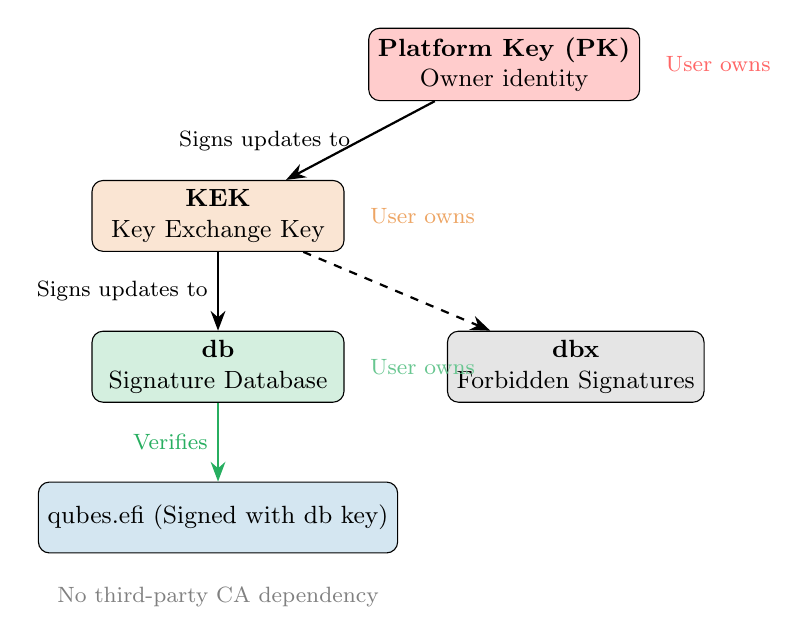
\begin{tikzpicture}[
    node distance=1.0cm,
    every node/.style={font=\small},
    key/.style={rectangle, draw, rounded corners, minimum width=3.2cm, minimum height=0.9cm, align=center},
    arrow/.style={-{Stealth[length=2.5mm]}, thick}
]
\node[key, fill=red!20] (pk) {\textbf{Platform Key (PK)}\\Owner identity};
\node[key, fill=warnorange!20, below left=1.0cm and 0.3cm of pk] (kek) {\textbf{KEK}\\Key Exchange Key};
\node[key, fill=securegreen!20, below=1.0cm of kek] (db) {\textbf{db}\\Signature Database};
\node[key, fill=gray!20, right=1.3cm of db] (dbx) {\textbf{dbx}\\Forbidden Signatures};
\node[key, fill=qubesblue!20, below=1.0cm of db] (uki) {qubes.efi (Signed with db key)};
\draw[arrow] (pk) -- node[left, font=\footnotesize, align=right] {Signs updates to} (kek);
\draw[arrow] (kek) -- node[left, font=\footnotesize, align=right] {Signs updates to} (db);
\draw[arrow, dashed] (kek) -- (dbx);
\draw[arrow, securegreen] (db) -- node[left, font=\footnotesize] {Verifies} (uki);
\node[right=0.2cm of pk, font=\footnotesize, text=red!60] {User owns};
\node[right=0.2cm of kek, font=\footnotesize, text=warnorange!70] {User owns};
\node[right=0.2cm of db, font=\footnotesize, text=securegreen!70] {User owns};
\node[below=0.3cm of uki, font=\footnotesize, text=gray, align=center] {No third-party CA dependency};
\end{tikzpicture}
\caption{UEFI Secure Boot key hierarchy. The user owns all keys.}
\label{fig:key-hierarchy}
\end{figure}

The \texttt{qubes-sb-keygen} subcommand generates the full PK/KEK/db hierarchy with configurable key parameters (RSA-2048 to RSA-4096, defaulting to RSA-4096). It produces EFI signature list (\texttt{.esl}) files, authenticated variable update (\texttt{.auth}) files, and step-by-step enrollment instructions for both \texttt{efi-updatevar} and \texttt{mokutil}.

\subsection{Update Hook and Atomic Replacement}

The update hook is a post-transaction RPM scriptlet that triggers on updates to \texttt{qubes-vmm-xen-unified} or \texttt{kernel-qubes-dom0}.

\begin{figure}[H]
\centering
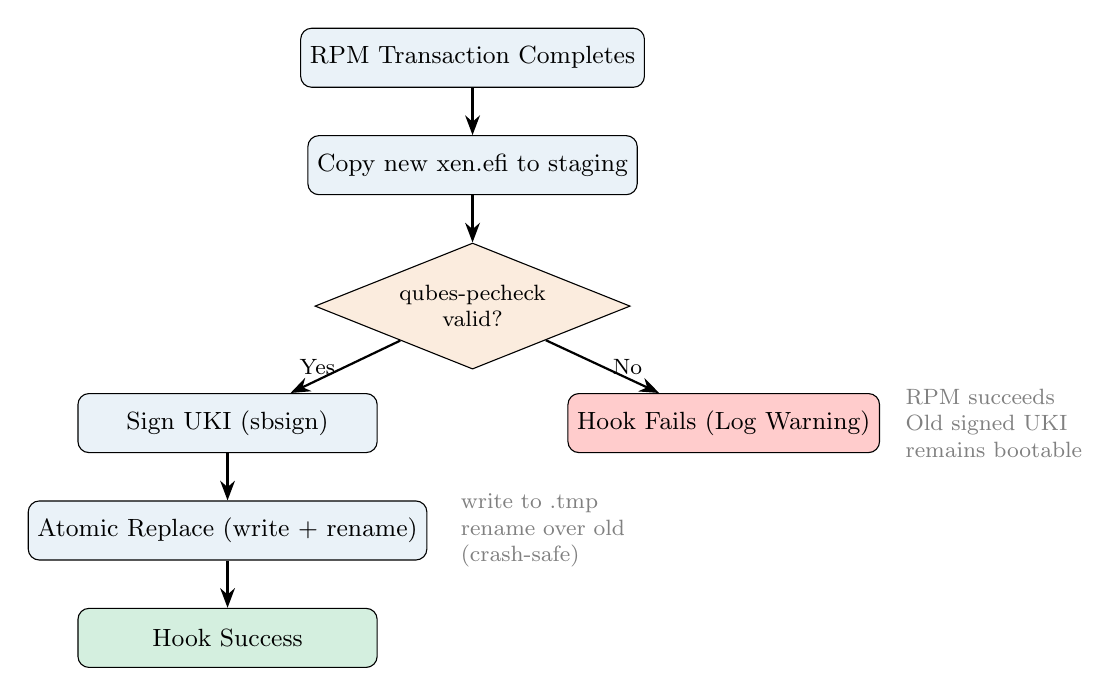
\begin{tikzpicture}[
    node distance=0.6cm,
    every node/.style={font=\small},
    process/.style={rectangle, draw, rounded corners, minimum width=3.8cm, minimum height=0.75cm, align=center, fill=qubesblue!10},
    decision/.style={diamond, draw, aspect=2.5, fill=warnorange!15, align=center, font=\footnotesize},
    arrow/.style={-{Stealth[length=2.5mm]}, thick}
]
\node[process] (update) {RPM Transaction Completes};
\node[process, below=of update] (copy) {Copy new xen.efi to staging};
\node[decision, below=of copy] (pecheck) {qubes-pecheck\\valid?};
\node[process, below left=0.7cm and 0.2cm of pecheck] (sign) {Sign UKI (sbsign)};
\node[process, below=of sign] (atomic) {Atomic Replace (write + rename)};
\node[process, below=of atomic, fill=securegreen!20] (done) {Hook Success};
\node[process, below right=0.7cm and 0.2cm of pecheck, fill=red!20] (fail) {Hook Fails (Log Warning)};
\draw[arrow] (update) -- (copy);
\draw[arrow] (copy) -- (pecheck);
\draw[arrow] (pecheck) -- node[left, font=\footnotesize] {Yes} (sign);
\draw[arrow] (pecheck) -- node[right, font=\footnotesize] {No} (fail);
\draw[arrow] (sign) -- (atomic);
\draw[arrow] (atomic) -- (done);
\node[right=0.2cm of fail, font=\footnotesize, text=gray, align=left] {RPM succeeds\\Old signed UKI\\remains bootable};
\node[right=0.3cm of atomic, font=\footnotesize, text=gray, align=left] {write to .tmp\\rename over old\\(crash-safe)};
\end{tikzpicture}
\caption{Update hook workflow. RPM installation always succeeds; signing failure leaves the previous UKI intact.}
\label{fig:update-hook}
\end{figure}

\textbf{Critical design decision:} The hook runs \textit{after} the RPM transaction completes. Package updates never fail due to signing issues. If signing fails, the hook logs a warning but the old signed UKI remains bootable. The atomic replacement writes to a temporary file then renames it over the active boot entry, ensuring crash safety.

\subsection{Fallback and Recovery}

\begin{figure}[H]
\centering
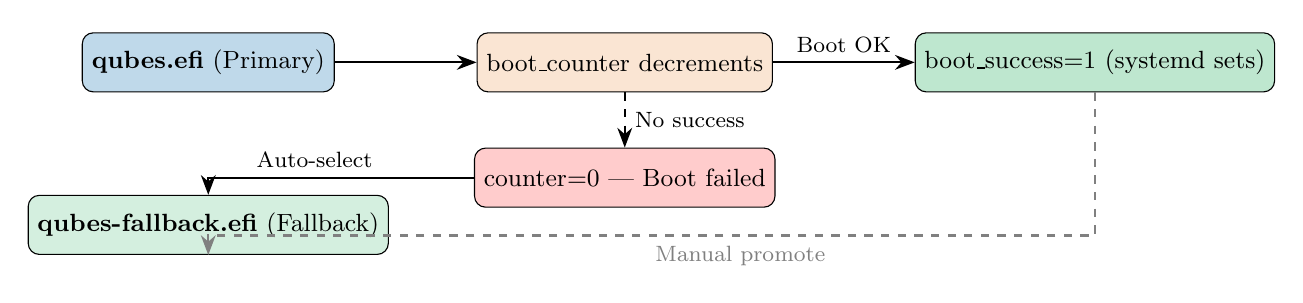
\begin{tikzpicture}[
    node distance=0.7cm and 1.8cm,
    every node/.style={font=\small},
    block/.style={rectangle, draw, rounded corners, minimum width=3.2cm, minimum height=0.75cm, align=center},
    arrow/.style={-{Stealth[length=2.5mm]}, thick}
]
\node[block, fill=qubesblue!30] (primary) {\textbf{qubes.efi} (Primary)};
\node[block, fill=securegreen!20, below=1.3cm of primary] (fallback) {\textbf{qubes-fallback.efi} (Fallback)};
\node[block, fill=warnorange!20, right=1.8cm of primary] (counter) {boot\_counter decrements};
\node[block, fill=securegreen!30, right=1.8cm of counter] (success) {boot\_success=1 (systemd sets)};
\node[block, fill=red!20, below=of counter] (fail) {counter=0 — Boot failed};
\draw[arrow] (primary) -- (counter);
\draw[arrow] (counter) -- node[above, font=\footnotesize] {Boot OK} (success);
\draw[arrow, dashed] (counter) -- node[right, font=\footnotesize] {No success} (fail);
\draw[arrow] (fail) -| node[above, font=\footnotesize, pos=0.3] {Auto-select} (fallback);
\draw[arrow, dashed, gray] (success) -- ++(0,-2.2) -| node[below, font=\footnotesize, pos=0.2, text=gray] {Manual promote} (fallback);
\end{tikzpicture}
\caption{Automatic fallback using GRUB boot\_counter/boot\_success variables.}
\label{fig:fallback}
\end{figure}

This project adapts Fedora's \href{https://fedoraproject.org/wiki/Changes/HiddenGrubMenu}{boot\_success mechanism} for UKI fallback selection. Qubes currently disables this mechanism; community bonding will investigate why (potential conflicts with Xen boot flow or hidden GRUB menu behavior) before re-enabling it for the UKI path. The \texttt{qubes-uki-promote-fallback} command will also exist for explicit promotion.

\textbf{Troubleshooting limitation:} UKI bundles prevent runtime parameter modification. For parameter debugging, users must either rebuild a debug UKI or temporarily disable Secure Boot. The documentation will cover both workflows.

\subsection{qubes-pecheck Fixes}

\textbf{False positive 1: \texttt{SizeOfRawData < VirtualSize}} --- The current check rejects Microsoft EFI binaries with this condition, which is valid per PE/COFF spec for BSS-style zero-filled sections. The fix only fails when \texttt{SizeOfRawData} is zero and \texttt{VirtualSize} is non-zero.

\textbf{False positive 2: \texttt{.linux} section flagged as non-executable} --- The \texttt{.linux} section carries the Dom0 kernel blob (data loaded by Xen, not PE-level code). The fix exempts well-known UKI data sections (\texttt{.linux}, \texttt{.initrd}, \texttt{.cmdline}) from the executable check. Both patches will be submitted during community bonding.

%---------------------------------------------------------------
% 4. CHALLENGES AND MITIGATIONS
%---------------------------------------------------------------
\section{Challenges and Mitigations}

\textbf{UEFI Variable Space Exhaustion:} Some firmware has limited NVRAM. Mitigation: check available space before enrollment, use compact \texttt{.esl} format, provide dry-run mode, document recovery procedures.

\textbf{OEM-Locked Firmware:} Some OEM firmware disallows custom PK replacement. Mitigation: support MOK path via \texttt{mokutil}/Shim, detect OEM-locked firmware and guide user to appropriate path.

\textbf{Signing Key Security:} Compromised key allows malicious UKI signing. Mitigation: document secure key storage (encrypted partition, hardware token), support offline signing workflows.

\textbf{Testing Environment Limitations:} QEMU/OVMF may not replicate all real firmware behavior. Mitigation: use OVMF for rapid iteration, validate on real hardware before midterm.

%---------------------------------------------------------------
% 5. TIMELINE
%---------------------------------------------------------------
\section{Timeline and Project Plan}

\begin{table}[H]
\centering
\small
\begin{tabular}{p{2.5cm} p{2.8cm} p{8cm}}
\toprule
\textbf{Date / Period} & \textbf{Phase} & \textbf{Detailed Sub-Tasks} \\
\midrule
May 1 -- May 26 & Community Bonding & Finalise \texttt{secureboot.conf} schema with Marek. Set up QEMU + OVMF. Submit \texttt{qubes-pecheck} patches. Investigate boot\_counter disable reason. Review \texttt{qubes-vmm-xen-unified} build scripts. \\
\midrule
Week 1--2 \newline (May 27 -- June 9) & Signing Core & Implement \texttt{qubes-uki-sign} wrapper around \texttt{sbsign}. Parse \texttt{secureboot.conf}. Unit tests with real unified binaries in QEMU/OVMF. \\
\midrule
Week 3--4 \newline (June 10 -- June 23) & Key Generation & Implement \texttt{qubes-sb-keygen}: configurable RSA key generation, \texttt{.esl}/\texttt{.auth} production. Test full sign-and-enroll cycle in OVMF. \\
\midrule
Week 5--6 \newline (June 24 -- July 7) & Update Hook & Implement RPM post-transaction hook. Add \texttt{qubes-pecheck} verification. Implement atomic replacement. Test full update cycle in QEMU. \\
\midrule
\textbf{July 8--11} & \textbf{Midterm} & \textbf{Deliverable:} Signing + key generation + update hook, end-to-end tested with real \texttt{qubes-vmm-xen-unified} binaries. \\
\midrule
Week 7--8 \newline (July 12 -- July 25) & Fallback UKI & Implement fallback generation and boot entry registration via \texttt{efibootmgr}. Implement \texttt{qubes-uki-promote-fallback}. Test recovery path in QEMU. \\
\midrule
Week 9--10 \newline (July 26 -- Aug 8) & Edge Cases \& UX & MOK path via \texttt{mokutil}. Handle: missing microcode, NVRAM exhaustion, failed \texttt{sbsign}. Begin user documentation. \\
\midrule
Week 11--12 \newline (Aug 9 -- Aug 22) & Docs \& Review & Complete user and developer documentation. Extended testing. Incorporate Marek's review feedback. \\
\midrule
Aug 22 -- Sep 1 & Buffer & Bug fixes, cleanup, final PR polish. \\
\bottomrule
\end{tabular}
\end{table}

\begin{figure}[H]
\centering
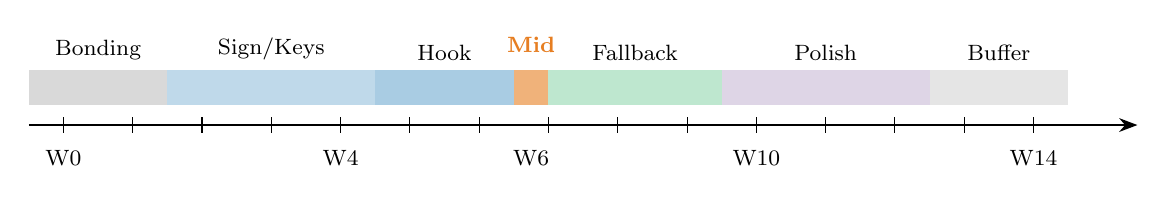
\begin{tikzpicture}[x=0.88cm, every node/.style={font=\footnotesize}]
\draw[thick, -{Stealth}] (0,0) -- (16,0);
\foreach \x in {0,1,...,14} { \draw (\x+0.5, 0.1) -- (\x+0.5, -0.1); }
\fill[gray!30] (0,0.25) rectangle (2,0.7);
\fill[qubesblue!30] (2,0.25) rectangle (5,0.7);
\fill[qubesblue!40] (5,0.25) rectangle (7,0.7);
\fill[warnorange!60] (7,0.25) rectangle (7.5,0.7);
\fill[securegreen!30] (7.5,0.25) rectangle (10,0.7);
\fill[xenpurple!20] (10,0.25) rectangle (13,0.7);
\fill[gray!20] (13,0.25) rectangle (15,0.7);
\node[above] at (1,0.7) {Bonding};
\node[above] at (3.5,0.7) {Sign/Keys};
\node[above] at (6,0.7) {Hook};
\node[above, text=warnorange] at (7.25,0.8) {\textbf{Mid}};
\node[above] at (8.75,0.7) {Fallback};
\node[above] at (11.5,0.7) {Polish};
\node[above] at (14,0.7) {Buffer};
\node[below] at (0.5,-0.2) {W0};
\node[below] at (4.5,-0.2) {W4};
\node[below] at (7.25,-0.2) {W6};
\node[below] at (10.5,-0.2) {W10};
\node[below] at (14.5,-0.2) {W14};
\end{tikzpicture}
\caption{GSoC timeline. Midterm at Week 6 delivers signing, key generation, and update integration.}
\label{fig:timeline}
\end{figure}

\subsection*{Exam Disclosure}
My end-semester exams at VJTI fall in May. Exact dates not yet released. I will communicate specific dates to Marek as soon as available and front-load bonding tasks accordingly.

\subsection*{Communication Plan}
\begin{itemize}
    \item \textbf{Weekly:} Formal progress update to \texttt{qubes-devel} every Monday covering completed work, next steps, and blockers
    \item \textbf{Ongoing:} Open PR/branch for incremental review. Responsive on Matrix and email within 24 hours
\end{itemize}

%---------------------------------------------------------------
% 6. ABOUT ME
%---------------------------------------------------------------
\section{About Me \& Commitments}

\subsection*{Basic Information}
\begin{itemize}
    \item \textbf{Name:} Harshit Bhalani
    \item \textbf{University:} Veermata Jijabai Technological Institute (VJTI), Mumbai, India
    \item \textbf{Major:} B.Tech in Electronics and Telecommunication Engineering (Second Year), Minor in Data Science
    \item \textbf{CGPA:} 9.02 / 10
    \item \textbf{GitHub:} \href{https://github.com/Harshit6-b}{github.com/Harshit6-b}
    \item \textbf{Email:} \href{mailto:harshitbhalani6@gmail.com}{harshitbhalani6@gmail.com}
    \item \textbf{Mailing lists:} Subscribed to \texttt{qubes-devel}
    \item \textbf{Core Stack:} Python, Bash, Verilog, C
\end{itemize}

\subsection*{Technical Background}

I am a second-year Electronics and Telecommunication Engineering student at VJTI Mumbai and a Core SY Member of the Society of Robotics and Automation (SRA-VJTI). My background is in digital hardware (RTL design in Verilog, FPGA development on Xilinx Artix-7, and embedded systems), but I work comfortably in Python and Bash, which are the primary languages for this project.

I came to this project through genuine study of the Qubes boot stack --- watching the Qubes OS Summit talks and the Xen Winter Meetup 2025, reading issues \#4371 and \#8206, and studying the UEFI specification before reaching out to Marek. Building understanding of the full UEFI boot sequence (SEC$\to$PEI$\to$DXE$\to$BDS$\to$TSL$\to$RT), the Secure Boot key hierarchy (PK/KEK/db/dbx), Shim/MOK, and PE/COFF format required significant self-directed effort.

\subsection*{Prior Contributions to Qubes OS}

\textbf{qubes-core-agent-linux PR \#644 --- Merged.}

Fixes a race condition in \texttt{qubes-firewall} (issues \href{https://github.com/QubesOS/qubes-issues/issues/3735}{\#3735}/\href{https://github.com/QubesOS/qubes-issues/issues/10643}{\#10643}). Root cause: \texttt{sd\_notify('READY=1')} fires before initialisation completes, causing SIGHUP to interrupt \texttt{qdb.read()} mid-protocol. An initial retry-loop fix was rejected because interrupting \texttt{qdb.read()} after sending a request desynchronises the QubesDB protocol. The approved approach uses \texttt{signal.pthread\_sigmask} to block SIGHUP/SIGTERM during all qdb operations.

\textbf{qubes-pecheck starter task --- Analysis complete, patches in progress.}

Ran \texttt{qubes-pecheck} against Microsoft, Ubuntu, openSUSE, and Arch UKI binaries. Identified two false positives described in the Implementation section. Patches are a community bonding goal.

\subsection*{Organization Specific Questions}

\textbf{Comfortable working independently with a remote mentor?} Yes. My entire interaction with Marek on PR \#644 has been asynchronous across time zones without difficulty. Weekly \texttt{qubes-devel} updates and an open PR branch will maintain full visibility.

\textbf{Native language?} Marathi, Hindi, and Gujarati. I communicate in English fluently with no concerns about technical communication with Marek.

\textbf{Submitting proposals to other organizations?} No. Qubes OS is my only application.

\subsection*{Commitments}
My university examinations conclude in May. I will treat this as a full-time commitment, dedicating a minimum of 40 hours per week throughout the GSoC coding period. This proposal has been reviewed by a senior member of SRA-VJTI before submission.

%---------------------------------------------------------------
% 7. REFERENCES
%---------------------------------------------------------------
\section{References}

\begin{itemize}
    \item Qubes Secure Boot Discussion: \href{https://github.com/QubesOS/qubes-issues/issues/4371}{Issue \#4371}
    \item Xen UKI Support: \href{https://github.com/QubesOS/qubes-issues/issues/8206}{Issue \#8206}
    \item Qubes Unified Xen: \href{https://github.com/QubesOS/qubes-vmm-xen-unified}{qubes-vmm-xen-unified repository}
    \item Fedora Boot Success Mechanism: \href{https://fedoraproject.org/wiki/Changes/HiddenGrubMenu}{Hidden GRUB Menu Change}
    \item UEFI Specification: \href{https://uefi.org/specifications}{uefi.org/specifications}
    \item Xen Unified Boot: \href{https://xenbits.xen.org/docs/unstable/misc/efi.html}{Xen EFI Documentation}
    \item PE/COFF Specification: \href{https://learn.microsoft.com/en-us/windows/win32/debug/pe-format}{Microsoft PE Format Documentation}
\end{itemize}

\end{document}
